\documentclass[10pt,showpacs,showkeys,%preprint,
amsfonts,amsmath,
onecolumn,
floatfix,aps,superscriptaddress]{revtex4}
\usepackage{amsfonts,amsmath,array}
\usepackage{graphicx}
\usepackage{bm}
%\usepackage{mal}
\usepackage{math}
\usepackage{cancel}
\begin{document}

\title{Multi Spectral Reduction of the Navier-Stokes equations}
\section{Purpose of this document}
This document contains notes for the application of multi-spectral
reduction to the Navier--Stokes equations, which will form the crux
of my thesis.

\section{Two dimensional Navier--Stokes}
What is particularly nice about two-dimensional turbulence is that the
we can represent the velocity by the vorticity, which has only one
non-zero component in two dimensions. The incompressible 2D Navier--Stokes
equations are:
\bec
\theNS, \quad \v\del\cdot\v{u}=0.
\eec
The vorticity is defined as 
$\v\omega = \del\times\v{u} = (\partial_x u_y - \partial_y u_x )\hat{\v{z}}$
Taking the Fourier transform, we have the following governing equation:
\begin{eqnarray}
  \frac{\partial \omega_{\v k}}{\partial t}
  + \nu_{\v k} \omega_{\v k} 
  &=& \int dp \int dq \frac{\epsilon_{\v{kpq}}}{\v q^2}
  \omega_{\v p}^* \omega_{\v q}^*
  + \v F_{\v k},
  \\
  \epsilon_{\v{kpq}} &=& \(\hat{\v z} \dot \v p \times \v q \)
  \delta\(\v k + \v p + \v q \)
\end{eqnarray}
where $\v F_{\v k}$ represents an external force. The 2D equations conserve
energy and enstrophy, so we would prefere a numerical scheme that maintains
this conservation. That is, the overlap between the two grids should give
identical values for the energy,
\begin{eqnarray}
  \label{E}
  E = \sum_i |u_i|^2,
\end{eqnarray}
and the enstrophy,
\begin{eqnarray}
  \label{Z}
  Z = \sum_i k_i^2|u_i|^2,
\end{eqnarray}
with appropriate weighting factors added for decimated grids.
We will see that enstrophy conservation, which involes the geometric 
quantity $\vk_i$, imposes a restriction on what types of grids we may use
and how we project between them.

One possible arrangement for the grids, wherein the coarse grid is 
twice as sparse and rotated by $45^\circ$,  
is given in figure \ref{grids}. In
the case where a coarse- and fine- grid point share the same location
in Fourier space, equation \eqref{Z} is automtically satisfied whenever
equation \eqref{E} is satisfied. In the arrangement given in figure \ref{grids},
half of the fine-grid nodes satisfy the property. For the projection operator to
conserve $E$ and $Z$, we thus need to transfer all of the energy and
enstrophy from the remaining fine-grid nodes to coarse grid nodes. 

\begin{figure}[htb]
  \begin{center}
    \includegraphics{grids}
    \caption{Grid layout for 2D NWSR. Red dots are for the fine grid, blue
crosses for the coarse grid. Note that the origin is excluded from both grids.}
    \label{grids}
  \end{center}
\end{figure}

\subsection{Spectrally Reduced Subgrids}
\subsubsection{Projection}
Each unmatched fine-grid point is surrounded by a (rotated) square of matched
coarse-grid points. This square constitutes the boundary of the region onto
which the energy and enstrophy of the fine-grid node will be distributed, 
cf: figure \ref{diamond}. Energy conservation is guaranteed if we 
set 
\begin{figure}[htb]
  \begin{center}
    \includegraphics{diamond}
    \caption{Projection diagram.}
    \label{diamond}
  \end{center}
\end{figure}
\begin{eqnarray}
  |u_1|^2 &=& \frac{\alpha}{2} |u|^2 
  \\
  |u_3|^2 &=& \frac{(1-\alpha)}{2} |u|^2 
  \\
  |u_0|^2 &=& \frac{\beta}{2} |u|^2 
  \\
  |u_2|^2 &=& \frac{(1-\beta)}{2} |u|^2.
\end{eqnarray}
The enstrophy balance equations are then
\begin{eqnarray}
  k_1^2 |u_1|^2 &=& \frac{\alpha}{2} k^2|u|^2 
  \\
  k_3^2|u_3|^2 &=& \frac{(1-\alpha)}{2} k^2|u|^2 
  \\
  k_0^2|u_0|^2 &=& \frac{\beta}{2} k^2|u|^2 
  \\
  k_2^2|u_2|^2 &=& \frac{(1-\beta)}{2} k^2|u|^2.
\end{eqnarray}
where $\vk_i$ is the wavevector for the coarse-grid mode $u_i$, $i=0,\dots,3$.
This is satisfied when
\begin{eqnarray}
  \alpha = \frac{k^2 -k_3^2}{ k_1^2 -k_3^2}
  \\
  \beta = \frac{k^2 -k_2^2}{ k_0^2 -k_2^2}.
\end{eqnarray}
The energy transferred from the central, fine-grid node to the surrounding
coarse grid points is
\begin{eqnarray}
  E_t=\alpha |u|^2 + (1-\alpha) |u|^2 + \beta |u|^2  (1-\beta) |u|^2 
  = |u|^2.
\end{eqnarray}
The enstrophy transferred is 
\begin{eqnarray}
  Z_t &=&
    k_1^2 \frac{\alpha}{2} |u|^2 +  k_3^2 \frac{(1-\alpha)}{2} |u|^2 +
  k_0^2 \frac{\beta}{2} |u|^2 +  k_2^2 \frac{(1-\beta)}{2} |u|^2
  \\ \nonumber
  &=&
  \half\[k_1^2 \frac{k^2 -k_3^2}{ k_1^2 -k_3^2}  
  +  k_3^2 \(1-\frac{k^2 -k_3^2}{ k_1^2 -k_3^2}\)  +
  k_0^2 \frac{k^2 -k_2^2}{ k_0^2 -k_2^2}  
  +  k_2^2 \(1-\frac{k^2 -k_2^2}{ k_0^2 -k_2^2}\)\] |u|^2
  \\ \nonumber
  &=& k^2 |u|^2
\end{eqnarray}
as required. 

Note that each of the coarse modes receives energy from the
fine grid mode that it coincides with as well as the projections
from two evactuated modes when the coarse mode lies within the region
covered by the fine grid. When the coarse mode lies at the boundary of
the fine grid, it receives contributions from just one find-grid mode.
See figure \ref{projside} for details.

\begin{figure}[htb]
  \begin{center}
    \includegraphics{projside}
    \caption{Side-view of projection.}
    \label{projside}
  \end{center}
\end{figure}

\subsubsection{Prolongation}
Once we have evolved the system on the coarse grid, 
we need to repopulate the modes that were evacuated by projection.
Since every coarse-grid mode has a corresponding fine-grid mode with
the same wavevector, the requirements of energy and enstrophy conservation
allow for a variety of repopulation schemes. 
Two obvious choices come immediately to mind:
\begin{enumerate}
\item
populate fine-gride modes with no corresponding coarse mode, using the inverse
of the projection operator to ensure conservation of invariants, 
\item
transfer all the energy from the coarse modes to the corresponding fine 
mode, setting all other modes to zero.
\end{enumerate}
An obvious choice is the combination of these two possibilities, using 
the ratio of fine-grid energies to determine how much energy is transferred
to what modes. The prolongation operator diagram is shown in figure 
\ref{prolside}, which gives the names of the modes that we will be using
in this subsection.
\begin{figure}[htb]
  \begin{center}
    \includegraphics{prolside}
    \caption{Side-view of projection.}
    \label{prolside}
  \end{center}
\end{figure}

\subsubsection{Prolongation choice 1}
An ideal solution would be to redistribute energies from the coarse grid
to the fine grid so that the original ratio of energies in the modes
of the fine grids is unaffected by the evolution of the coarse grid.
That is, a coarse mode $U_+$ was populated with energy with ratio 
$E_0:E_+:E_{++}$, with energy from the fine-grid modes $u_0$, $u_+$, 
and $u_{++}$, respectively, i.e.\ , before projection, we had
\begin{eqnarray}
  E_0:E_+:E_{++} = u_0^2: u_+^2: u_{++}^2
\end{eqnarray}
and we would like to ensure that this is the case after prolongation. 

However, energy and enstrophy conservation relies on energies being 
distributed in ratios $\alpha$ and $(1-\alpha)$, which may be impossible if,
for example, if only one of $U_-$ and $U_+$ drops to zero.

\subsubsection{Prolongation choice 2}
During projection, the energy of mode $U_-$ is determined by the 
geometric factors $\alpha_i$ and the energies of the fine-grid modes.
That is,
\begin{eqnarray}
  U_-^2 &=& \(1-\alpha_{--}\)E_{--} + E_- + \alpha_0E_0
  \\
  U_+^2 &=& \(1-\alpha_0\)E_0 + E_+ + \alpha_{++}E_{++}.
\end{eqnarray}
Let $\hat U_i$ denote $U_i$ after the completion of a Runge--Kutta time step.
From this, we can determine the energy that the fine modes should have.
We choose to remove energy from $U_-$ and $U_+$ so that
\begin{eqnarray}
  u_0^2= E_0 \leftarrow u_0^2 \times
  \min\{\frac{\hat U_-^2}{U_-^2},\frac{\hat U_+^2}{U_+^2}\}.
\end{eqnarray}
This guarantees that we do not attempt to remove more energy from coarse
modes than there be present. Any remaining energy is then deposited into 
the fine-grid modes that coincide with coarse-grid modes in Fourier space, 
which automatically conserves both $E$ and $Z$.

\subsubsection{Spectral Reduction of Governing Equations}
Now we have to figure out what the hell to do with the coarse grid.

\subsection{Scaled Subgrids}
Shell models of turbulence spectrally reduce in a special case, since
the GOY model reduced to the DN model, which is then a fixed point. Id
est, the nonlinear source term is invariant.  Unsurprisingly, the
Navier--Stokes equations present a more difficult problem for spectral 
reduction, because the binning of modes removes the perfectly triadic 
interaction between wavemodes.  

\subsubsection{The Spectrally-scaled Navier--Stokes equations}
However, this is not the only map that we may apply to the governing
equation. Taking the spectral vorticity Navier--Stokes equations, each
mode $\v\omega_{\v k}$ has $\v{k} \in \{k_0\(i,j\),i,j=1,\dots ,n \}$, where
$k_0$ is the inverse scale of the $x$-space system, i.e.\ 
$\v{x}\in (0,\pi/k_0)\times(0,\pi/k_0)$ (in our not-really-applied fashion,
we typically take $k_0=1$).  

Let $k_0^{(0)}$ be the spacing of the fine 
grid, and $k_0^{(1)}=2k_0^{(0)}$ be the subgrid spacing, as in 
figure~\ref{bb_grids}. The subgrid has 
$\v{k} \in \{2k_0\(i,j\),i,j=1,\dots ,n \}$, which corresponds to 
$\v{x}\in (0,\pi/(2k_0))\times(0,\pi/(2k_0))$. This is equivalent to 
the scaling $\v{x} \rightarrow \v{x}/2$.  If we want to simulate a fluid 
on $\v{x}\in (0,\pi/(k_0))\times(0,\pi/(k_0))$, we simply rescale $\v{x}$ by
a factor of two. This is equivalent to modifying the Navier--Stokes equations
from
\be
\theNS
\ee
to
\be
\ppt{\v{u}} +2\v{u}\cdot\grad\v{u} 
= -\frac{1}{\rho}2\grad P + 4\nu\nabla^2 \v{u}+ \v{F}.
\ee


The primary advantage of this technique is that it leaves the form of the
governing equation the same.  Thus, all of the computational techniques that 
we have developped for simulating the undecimated Navier--Stokes equations
can still be applied.

\begin{figure}[htb]
  \begin{center}
    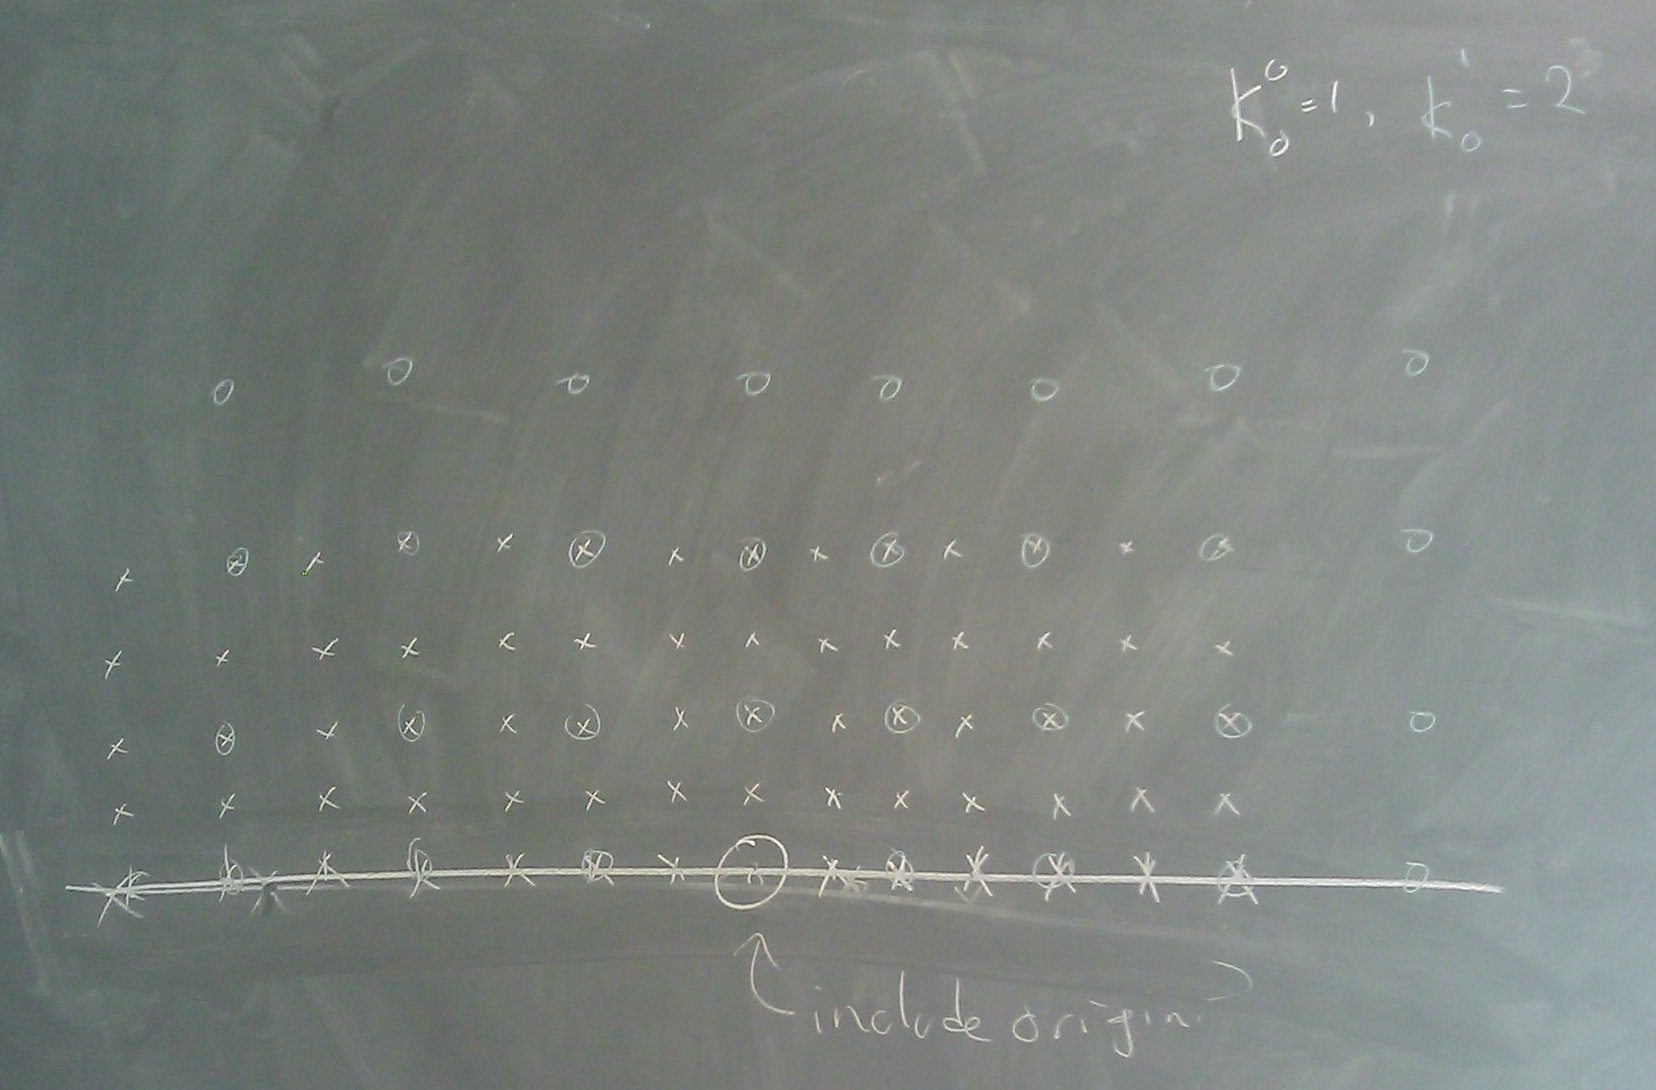
\includegraphics[height=60mm]{bb_grids.jpg}
    \caption{Scaled Subgrid diagram}
    \label{bb_grids}
  \end{center}
\end{figure}

\subsubsection{Grids}
However, scaling the grids by a factor introduces a restriction on the geometry
that we can use. In particular, the imposition of a square latticewill lead
to a problem with projection/prolongation near the spectral origin: fine-grid 
modes adjacent to the origin can only project their energy onto coarse modes
with higher wavenumber, which breaks enstrophy conservation. This may be 
rectified by reintroducing the spectral origin, which is not evolved by the
spectral Navier--Stokes equations, as a buffer into which some energy may be
depositied.  In this case, every fine-grid mode is has at least one adjacent
coarse-grid mode with higher $k$ and one adjacent coarse-grid mode with lower
$k$.

TODO: show projections.  Also, what about prolonging the boundary modes?

\end{document}
